% Created 2023-12-03 So 16:34
% Intended LaTeX compiler: pdflatex
\documentclass[11pt]{article}
\usepackage[utf8]{inputenc}
\usepackage{lmodern}
\usepackage[T1]{fontenc}
\usepackage{textcomp}
\usepackage{graphicx}
\usepackage{longtable}
\usepackage{wrapfig}
\usepackage{rotating}
\usepackage[normalem]{ulem}
\usepackage{amsmath}
\usepackage{amssymb}
\usepackage{capt-of}
\usepackage{hyperref}
\usepackage{verbatim}
\usepackage{listings}
\usepackage{underscore}
\author{Leon Schwarzäugl}
\date{\today}
\title{Computational Science on Many-Core Architectures \\Exercise 9}
\hypersetup{
 pdfauthor={Leon Schwarzäugl},
 pdftitle={Computational Science on Many-Core Architectures, Exercise 9},
 pdfkeywords={},
 pdfsubject={},
 pdfcreator={Emacs 30.0.50 (Org mode 9.6.12)},
 pdflang={English}}
\begin{document}
\maketitle
The code for all tasks can be found at: \url{https://github.com/Swarsel/CSE_TUWIEN/tree/main/WS2023/Many-Core%20Architectures/e9}

\newpage
\section{Libraries}

I tried to implement the dot product for all four libraries (they can be found in the respective 1a-1d files in the linked git repository). \\
Sadly I failed to produce working implementations for Thrust and ViennaCL; for Thrust, I got a very long error message that I was not able to handle:

\begin{tiny}
\begin{verbatim}
In file included from ea00eecd.cu:6:
In file included from /usr/include/thrust/device_vector.h:25:
In file included from /usr/include/thrust/detail/vector_base.h:29:
In file included from /usr/include/thrust/detail/contiguous_storage.h:240:
In file included from /usr/include/thrust/detail/contiguous_storage.inl:22:
In file included from /usr/include/thrust/detail/allocator/copy_construct_range.h:46:
In file included from /usr/include/thrust/detail/allocator/copy_construct_range.inl:21:
In file included from /usr/include/thrust/detail/copy.h:90:
In file included from /usr/include/thrust/detail/copy.inl:22:
In file included from /usr/include/thrust/system/detail/adl/copy.h:25:
In file included from /usr/include/thrust/system/detail/sequential/copy.h:62:
/usr/include/thrust/system/detail/sequential/copy.inl:115:18: error: __host__ function 'copy' cannot overload __host__ __device__ function 'copy'
  OutputIterator copy(sequential::execution_policy<DerivedPolicy> &,
[...]
\end{verbatim}
\end{tiny}
For ViennaCL, I got this weird, seemingly HIP-related error:

\begin{tiny}
\begin{verbatim}
In file included from a7344771.cu:7:
In file included from ./viennacl/vector.hpp:27:
In file included from ./viennacl/detail/vector_def.hpp:26:
In file included from ./viennacl/tools/entry_proxy.hpp:27:
In file included from ./viennacl/scalar.hpp:30:
In file included from ./viennacl/linalg/scalar_operations.hpp:40:
./viennacl/linalg/cuda/scalar_operations.hpp:88:12: error: use of undeclared identifier __hipPushCallConfiguration
  as_kernel<<<1, 1>>>(viennacl::cuda_arg(s1),
[...]
\end{verbatim}
\end{tiny}

I fear these errors arose because of some oversight on my part; however, I house a small hope that there might be something wrong with the remote host. This is because when I tried to run my CUDA dot product, I got another error. This code ran without issue for the last exercise, and all of the non-working libraries are using CUDA.

\begin{tiny}
\begin{verbatim}
In file included from e1fb6cf3.cu:1:
./cuda_errchk.hpp:4:35: error: unknown type name 'cudaError'
inline void cuda_error_check_impl(cudaError error_code, const int line )
                                  ^
./cuda_errchk.hpp:6:7: error: use of undeclared identifier 'cudaSuccess'
  if (cudaSuccess != error_code)
[...]
\end{verbatim}
\end{tiny}

\newpage
As for the comparison, this data shines a grim light, as both of these libraries are a lot slower than the OpenCL approach from last week (the Thrust, ViennaCL and CUDA implementations are omitted in the graph due to the above problems - however, I included a file csmca_1_all(broken).py that would theoretically perform a full benchmark for completeness). \\

I have the feeling that for the two libraries that I got to work (Boost and VexCL) I also made some mistake, it seems unlikely that these libraries perform so poorly for such a simple task. I wish I had more time to investigate this matter more, but due to a lot of projects being due I did not have the time to do that :(

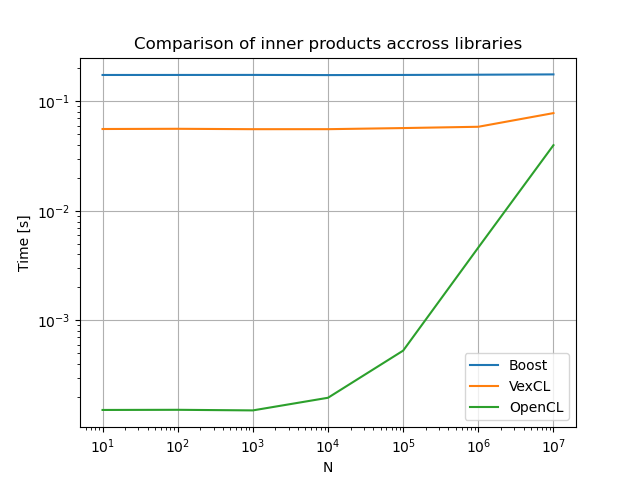
\includegraphics[scale=0.6]{plots/1.png}

\section{HIP}

Sadly, the problems do not end here. I also tried to implement this by following the slides (pages 3 and 4 of slide set B) very precicely. My attempt can be found in the file 2.cpp in the git repository. This just ended in a Segmentation Fault however, so I fear that this time I am fully at fault. Again here, I did not find the time to fix this problem.\\

Sadly this also means that I do not have any (relevant) plots or comparisons to show for this one. Again, in the git repository is a theoretical benchmark file (csmca_2(broken).py) that I figure would work if the code would work in general.

\end{document}
